\fancyhf{}
\fancyfoot[L]{\deflfoot{}}% Custom footer
\fancyfoot[R]{\defrfoot{}}% Custom footer
\renewcommand{\headrulewidth}{0pt}% Line at the header visible
%

\includegraphics[height=3.5cm]{Logo3rd.png} \hfill 
\includegraphics[height=3cm]{319th.png}%
%
\begin{flushright}Le \today{} à \currenttime{}\end{flushright}%
%
%\vfil%
%
\section*{Lettre de publication}%
\phantomsection%
\addcontentsline{toc}{section}{\protect\numberline{}Lettre de publication}%
%
\vfil%
%
\docname{} est publié par l'État Major (EM) du \rgt{}.%
%
\vfil%
%
Le \rgt{} est un escadron évoluant sur le simulateur de combat \dcs{} (DCS), édité par ``Eagle Dynamics'' (ED), membre de l'escadrille virtuelle francophone \thirdwing{}.
%
\vfil%
%
% Ce document n'engage aucune partie autre que le \rgt{}.
%
%\vfil%
%
Ce document peut être transmis à tous les membres de la 3rd Wing sans autorisation préalable, ou à d'autres personnes membres d'un escadron évoluant sur DCS.
%
\vfil%
%
Un membre de l'EM du \rgt{} doit être averti lorsque ce document est transmis à un membre d'un autre escadron évoluant sous DCS.
%
\vfil%
%
Les commentaires ou suggestions à propos de ce document peuvent être envoyés à: \href{mailto:etcher3rd@gmail.com}{etcher3rd@gmail.com}.
%
\vfil%
%
\begin{flushright}
    \hfill \parbox{0.3\textwidth}{\raggedright \hfill 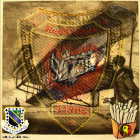
\includegraphics[width=0.1\textwidth]{avatar.png}} \hfil \parbox{0.4\textwidth}{\raggedright etcher \\ Cpt, 319th Rgt \\ \inmem{}}%
%    
\vfil%
%
\hfill \parbox{0.3\textwidth}{\raggedright \hfill } \hfil \parbox{0.4\textwidth}%
{\centering \includegraphics[width=0.37\textwidth]{signature.png}\par}%   
\end{flushright}%
%
\vfil%